
%% bare_jrnl.tex
%% V1.3
%% 2007/01/11
%% by Michael Shell
%% see http://www.michaelshell.org/
%% for current contact information.
%%
%% This is a skeleton file demonstrating the use of IEEEtran.cls
%% (requires IEEEtran.cls version 1.7 or later) with an IEEE journal paper.
%%
%% Support sites:
%% http://www.michaelshell.org/tex/ieeetran/
%% http://www.ctan.org/tex-archive/macros/latex/contrib/IEEEtran/
%% and
%% http://www.ieee.org/



% *** Authors should verify (and, if needed, correct) their LaTeX system  ***
% *** with the testflow diagnostic prior to trusting their LaTeX platform ***
% *** with production work. IEEE's font choices can trigger bugs that do  ***
% *** not appear when using other class files.                            ***
% The testflow support page is at:
% http://www.michaelshell.org/tex/testflow/


%%*************************************************************************
%% Legal Notice:
%% This code is offered as-is without any warranty either expressed or
%% implied; without even the implied warranty of MERCHANTABILITY or
%% FITNESS FOR A PARTICULAR PURPOSE! 
%% User assumes all risk.
%% In no event shall IEEE or any contributor to this code be liable for
%% any damages or losses, including, but not limited to, incidental,
%% consequential, or any other damages, resulting from the use or misuse
%% of any information contained here.
%%
%% All comments are the opinions of their respective authors and are not
%% necessarily endorsed by the IEEE.
%%
%% This work is distributed under the LaTeX Project Public License (LPPL)
%% ( http://www.latex-project.org/ ) version 1.3, and may be freely used,
%% distributed and modified. A copy of the LPPL, version 1.3, is included
%% in the base LaTeX documentation of all distributions of LaTeX released
%% 2003/12/01 or later.
%% Retain all contribution notices and credits.
%% ** Modified files should be clearly indicated as such, including  **
%% ** renaming them and changing author support contact information. **
%%
%% File list of work: IEEEtran.cls, IEEEtran_HOWTO.pdf, bare_adv.tex,
%%                    bare_conf.tex, bare_jrnl.tex, bare_jrnl_compsoc.tex
%%*************************************************************************

% Note that the a4paper option is mainly intended so that authors in
% countries using A4 can easily print to A4 and see how their papers will
% look in print - the typesetting of the document will not typically be
% affected with changes in paper size (but the bottom and side margins will).
% Use the testflow package mentioned above to verify correct handling of
% both paper sizes by the user's LaTeX system.
%
% Also note that the "draftcls" or "draftclsnofoot", not "draft", option
% should be used if it is desired that the figures are to be displayed in
% draft mode.
%
\documentclass[journal]{IEEEtran}
\usepackage{blindtext}
\usepackage{graphicx}
\usepackage{amsmath}

% Some very useful LaTeX packages include:
% (uncomment the ones you want to load)


% *** MISC UTILITY PACKAGES ***
%
%\usepackage{ifpdf}
% Heiko Oberdiek's ifpdf.sty is very useful if you need conditional
% compilation based on whether the output is pdf or dvi.
% usage:
% \ifpdf
%   % pdf code
% \else
%   % dvi code
% \fi
% The latest version of ifpdf.sty can be obtained from:
% http://www.ctan.org/tex-archive/macros/latex/contrib/oberdiek/
% Also, note that IEEEtran.cls V1.7 and later provides a builtin
% \ifCLASSINFOpdf conditional that works the same way.
% When switching from latex to pdflatex and vice-versa, the compiler may
% have to be run twice to clear warning/error messages.






% *** CITATION PACKAGES ***
%
%\usepackage{cite}
% cite.sty was written by Donald Arseneau
% V1.6 and later of IEEEtran pre-defines the format of the cite.sty package
% \cite{} output to follow that of IEEE. Loading the cite package will
% result in citation numbers being automatically sorted and properly
% "compressed/ranged". e.g., [1], [9], [2], [7], [5], [6] without using
% cite.sty will become [1], [2], [5]--[7], [9] using cite.sty. cite.sty's
% \cite will automatically add leading space, if needed. Use cite.sty's
% noadjust option (cite.sty V3.8 and later) if you want to turn this off.
% cite.sty is already installed on most LaTeX systems. Be sure and use
% version 4.0 (2003-05-27) and later if using hyperref.sty. cite.sty does
% not currently provide for hyperlinked citations.
% The latest version can be obtained at:
% http://www.ctan.org/tex-archive/macros/latex/contrib/cite/
% The documentation is contained in the cite.sty file itself.






% *** GRAPHICS RELATED PACKAGES ***
%
\ifCLASSINFOpdf
  % \usepackage[pdftex]{graphicx}
  % declare the path(s) where your graphic files are
  % \graphicspath{{../pdf/}{../jpeg/}}
  % and their extensions so you won't have to specify these with
  % every instance of \includegraphics
  % \DeclareGraphicsExtensions{.pdf,.jpeg,.png}
\else
  % or other class option (dvipsone, dvipdf, if not using dvips). graphicx
  % will default to the driver specified in the system graphics.cfg if no
  % driver is specified.
  % \usepackage[dvips]{graphicx}
  % declare the path(s) where your graphic files are
  % \graphicspath{{../eps/}}
  % and their extensions so you won't have to specify these with
  % every instance of \includegraphics
  % \DeclareGraphicsExtensions{.eps}
\fi
% graphicx was written by David Carlisle and Sebastian Rahtz. It is
% required if you want graphics, photos, etc. graphicx.sty is already
% installed on most LaTeX systems. The latest version and documentation can
% be obtained at: 
% http://www.ctan.org/tex-archive/macros/latex/required/graphics/
% Another good source of documentation is "Using Imported Graphics in
% LaTeX2e" by Keith Reckdahl which can be found as epslatex.ps or
% epslatex.pdf at: http://www.ctan.org/tex-archive/info/
%
% latex, and pdflatex in dvi mode, support graphics in encapsulated
% postscript (.eps) format. pdflatex in pdf mode supports graphics
% in .pdf, .jpeg, .png and .mps (metapost) formats. Users should ensure
% that all non-photo figures use a vector format (.eps, .pdf, .mps) and
% not a bitmapped formats (.jpeg, .png). IEEE frowns on bitmapped formats
% which can result in "jaggedy"/blurry rendering of lines and letters as
% well as large increases in file sizes.
%
% You can find documentation about the pdfTeX application at:
% http://www.tug.org/applications/pdftex





% *** MATH PACKAGES ***
%
%\usepackage[cmex10]{amsmath}
% A popular package from the American Mathematical Society that provides
% many useful and powerful commands for dealing with mathematics. If using
% it, be sure to load this package with the cmex10 option to ensure that
% only type 1 fonts will utilized at all point sizes. Without this option,
% it is possible that some math symbols, particularly those within
% footnotes, will be rendered in bitmap form which will result in a
% document that can not be IEEE Xplore compliant!
%
% Also, note that the amsmath package sets \interdisplaylinepenalty to 10000
% thus preventing page breaks from occurring within multiline equations. Use:
%\interdisplaylinepenalty=2500
% after loading amsmath to restore such page breaks as IEEEtran.cls normally
% does. amsmath.sty is already installed on most LaTeX systems. The latest
% version and documentation can be obtained at:
% http://www.ctan.org/tex-archive/macros/latex/required/amslatex/math/





% *** SPECIALIZED LIST PACKAGES ***
%
%\usepackage{algorithmic}
% algorithmic.sty was written by Peter Williams and Rogerio Brito.
% This package provides an algorithmic environment fo describing algorithms.
% You can use the algorithmic environment in-text or within a figure
% environment to provide for a floating algorithm. Do NOT use the algorithm
% floating environment provided by algorithm.sty (by the same authors) or
% algorithm2e.sty (by Christophe Fiorio) as IEEE does not use dedicated
% algorithm float types and packages that provide these will not provide
% correct IEEE style captions. The latest version and documentation of
% algorithmic.sty can be obtained at:
% http://www.ctan.org/tex-archive/macros/latex/contrib/algorithms/
% There is also a support site at:
% http://algorithms.berlios.de/index.html
% Also of interest may be the (relatively newer and more customizable)
% algorithmicx.sty package by Szasz Janos:
% http://www.ctan.org/tex-archive/macros/latex/contrib/algorithmicx/




% *** ALIGNMENT PACKAGES ***
%
%\usepackage{array}
% Frank Mittelbach's and David Carlisle's array.sty patches and improves
% the standard LaTeX2e array and tabular environments to provide better
% appearance and additional user controls. As the default LaTeX2e table
% generation code is lacking to the point of almost being broken with
% respect to the quality of the end results, all users are strongly
% advised to use an enhanced (at the very least that provided by array.sty)
% set of table tools. array.sty is already installed on most systems. The
% latest version and documentation can be obtained at:
% http://www.ctan.org/tex-archive/macros/latex/required/tools/


%\usepackage{mdwmath}
%\usepackage{mdwtab}
% Also highly recommended is Mark Wooding's extremely powerful MDW tools,
% especially mdwmath.sty and mdwtab.sty which are used to format equations
% and tables, respectively. The MDWtools set is already installed on most
% LaTeX systems. The lastest version and documentation is available at:
% http://www.ctan.org/tex-archive/macros/latex/contrib/mdwtools/


% IEEEtran contains the IEEEeqnarray family of commands that can be used to
% generate multiline equations as well as matrices, tables, etc., of high
% quality.


%\usepackage{eqparbox}
% Also of notable interest is Scott Pakin's eqparbox package for creating
% (automatically sized) equal width boxes - aka "natural width parboxes".
% Available at:
% http://www.ctan.org/tex-archive/macros/latex/contrib/eqparbox/





% *** SUBFIGURE PACKAGES ***
%\usepackage[tight,footnotesize]{subfigure}
% subfigure.sty was written by Steven Douglas Cochran. This package makes it
% easy to put subfigures in your figures. e.g., "Figure 1a and 1b". For IEEE
% work, it is a good idea to load it with the tight package option to reduce
% the amount of white space around the subfigures. subfigure.sty is already
% installed on most LaTeX systems. The latest version and documentation can
% be obtained at:
% http://www.ctan.org/tex-archive/obsolete/macros/latex/contrib/subfigure/
% subfigure.sty has been superceeded by subfig.sty.



%\usepackage[caption=false]{caption}
%\usepackage[font=footnotesize]{subfig}
% subfig.sty, also written by Steven Douglas Cochran, is the modern
% replacement for subfigure.sty. However, subfig.sty requires and
% automatically loads Axel Sommerfeldt's caption.sty which will override
% IEEEtran.cls handling of captions and this will result in nonIEEE style
% figure/table captions. To prevent this problem, be sure and preload
% caption.sty with its "caption=false" package option. This is will preserve
% IEEEtran.cls handing of captions. Version 1.3 (2005/06/28) and later 
% (recommended due to many improvements over 1.2) of subfig.sty supports
% the caption=false option directly:
%\usepackage[caption=false,font=footnotesize]{subfig}
%
% The latest version and documentation can be obtained at:
% http://www.ctan.org/tex-archive/macros/latex/contrib/subfig/
% The latest version and documentation of caption.sty can be obtained at:
% http://www.ctan.org/tex-archive/macros/latex/contrib/caption/




% *** FLOAT PACKAGES ***
%
%\usepackage{fixltx2e}
% fixltx2e, the successor to the earlier fix2col.sty, was written by
% Frank Mittelbach and David Carlisle. This package corrects a few problems
% in the LaTeX2e kernel, the most notable of which is that in current
% LaTeX2e releases, the ordering of single and double column floats is not
% guaranteed to be preserved. Thus, an unpatched LaTeX2e can allow a
% single column figure to be placed prior to an earlier double column
% figure. The latest version and documentation can be found at:
% http://www.ctan.org/tex-archive/macros/latex/base/



%\usepackage{stfloats}
% stfloats.sty was written by Sigitas Tolusis. This package gives LaTeX2e
% the ability to do double column floats at the bottom of the page as well
% as the top. (e.g., "\begin{figure*}[!b]" is not normally possible in
% LaTeX2e). It also provides a command:
%\fnbelowfloat
% to enable the placement of footnotes below bottom floats (the standard
% LaTeX2e kernel puts them above bottom floats). This is an invasive package
% which rewrites many portions of the LaTeX2e float routines. It may not work
% with other packages that modify the LaTeX2e float routines. The latest
% version and documentation can be obtained at:
% http://www.ctan.org/tex-archive/macros/latex/contrib/sttools/
% Documentation is contained in the stfloats.sty comments as well as in the
% presfull.pdf file. Do not use the stfloats baselinefloat ability as IEEE
% does not allow \baselineskip to stretch. Authors submitting work to the
% IEEE should note that IEEE rarely uses double column equations and
% that authors should try to avoid such use. Do not be tempted to use the
% cuted.sty or midfloat.sty packages (also by Sigitas Tolusis) as IEEE does
% not format its papers in such ways.


%\ifCLASSOPTIONcaptionsoff
%  \usepackage[nomarkers]{endfloat}
% \let\MYoriglatexcaption\caption
% \renewcommand{\caption}[2][\relax]{\MYoriglatexcaption[#2]{#2}}
%\fi
% endfloat.sty was written by James Darrell McCauley and Jeff Goldberg.
% This package may be useful when used in conjunction with IEEEtran.cls'
% captionsoff option. Some IEEE journals/societies require that submissions
% have lists of figures/tables at the end of the paper and that
% figures/tables without any captions are placed on a page by themselves at
% the end of the document. If needed, the draftcls IEEEtran class option or
% \CLASSINPUTbaselinestretch interface can be used to increase the line
% spacing as well. Be sure and use the nomarkers option of endfloat to
% prevent endfloat from "marking" where the figures would have been placed
% in the text. The two hack lines of code above are a slight modification of
% that suggested by in the endfloat docs (section 8.3.1) to ensure that
% the full captions always appear in the list of figures/tables - even if
% the user used the short optional argument of \caption[]{}.
% IEEE papers do not typically make use of \caption[]'s optional argument,
% so this should not be an issue. A similar trick can be used to disable
% captions of packages such as subfig.sty that lack options to turn off
% the subcaptions:
% For subfig.sty:
% \let\MYorigsubfloat\subfloat
% \renewcommand{\subfloat}[2][\relax]{\MYorigsubfloat[]{#2}}
% For subfigure.sty:
% \let\MYorigsubfigure\subfigure
% \renewcommand{\subfigure}[2][\relax]{\MYorigsubfigure[]{#2}}
% However, the above trick will not work if both optional arguments of
% the \subfloat/subfig command are used. Furthermore, there needs to be a
% description of each subfigure *somewhere* and endfloat does not add
% subfigure captions to its list of figures. Thus, the best approach is to
% avoid the use of subfigure captions (many IEEE journals avoid them anyway)
% and instead reference/explain all the subfigures within the main caption.
% The latest version of endfloat.sty and its documentation can obtained at:
% http://www.ctan.org/tex-archive/macros/latex/contrib/endfloat/
%
% The IEEEtran \ifCLASSOPTIONcaptionsoff conditional can also be used
% later in the document, say, to conditionally put the References on a 
% page by themselves.





% *** PDF, URL AND HYPERLINK PACKAGES ***
%
%\usepackage{url}
% url.sty was written by Donald Arseneau. It provides better support for
% handling and breaking URLs. url.sty is already installed on most LaTeX
% systems. The latest version can be obtained at:
% http://www.ctan.org/tex-archive/macros/latex/contrib/misc/
% Read the url.sty source comments for usage information. Basically,
% \url{my_url_here}.





% *** Do not adjust lengths that control margins, column widths, etc. ***
% *** Do not use packages that alter fonts (such as pslatex).         ***
% There should be no need to do such things with IEEEtran.cls V1.6 and later.
% (Unless specifically asked to do so by the journal or conference you plan
% to submit to, of course. )


% correct bad hyphenation here
\hyphenation{}


\begin{document}
%
% paper title
% can use linebreaks \\ within to get better formatting as desired
\title{Modeling Temperature Profile of Solar Corona at Microwave and Radiowave Frequencies}
%
%
% author names and IEEE memberships
% note positions of commas and nonbreaking spaces ( ~ ) LaTeX will not break
% a structure at a ~ so this keeps an author's name from being broken across
% two lines.
% use \thanks{} to gain access to the first footnote area
% a separate \thanks must be used for each paragraph as LaTeX2e's \thanks
% was not built to handle multiple paragraphs
%


\author{Pranav Sankhe \emph{EE Dept. IIT Bombay}, Prof R.K.Shevgaonkar \emph{EE Dept. IIT Bombay}
                % <-this % stops a space
\thanks{Professor R.K.Shevgaonkar is a professor at Department
of Electrical Engineering, Indian Institute of Technology, Bombay.}% <-this % stops a space
%\thanks{J. Doe and J. Doe are with Anonymous University.}% <-this % stops a space
%\thanks{Manuscript received April 19, 2005; revised January 11, 2007.}}
}
% note the % following the last \IEEEmembership and also \thanks - 
% these prevent an unwanted space from occurring between the last author name
% and the end of the author line. i.e., if you had this:
% 
% \author{....lastname \thanks{...} \thanks{...} }
%                     ^------------^------------^----Do not want these spaces!
%
% a space would be appended to the last name and could cause every name on that
% line to be shifted left slightly. This is one of those "LaTeX things". For
% instance, "\textbf{A} \textbf{B}" will typeset as "A B" not "AB". To get
% "AB" then you have to do: "\textbf{A}\textbf{B}"
% \thanks is no different in this regard, so shield the last } of each \thanks
% that ends a line with a % and do not let a space in before the next \thanks.
% Spaces after \IEEEmembership other than the last one are OK (and needed) as
% you are supposed to have spaces between the names. For what it is worth,
% this is a minor point as most people would not even notice if the said evil
% space somehow managed to creep in.



% The paper headers
%\markboth{Journal of \LaTeX\ Class Files,~Vol.~6, No.~1, January~2007}%
%{Shell \MakeLowercase{\textit{et al.}}: Bare Demo of IEEEtran.cls for Journals}
% The only time the second header will appear is for the odd numbered pages
% after the title page when using the twoside option.
% 
% *** Note that you probably will NOT want to include the author's ***
% *** name in the headers of peer review papers.                   ***
% You can use \ifCLASSOPTIONpeerreview for conditional compilation here if
% you desire.




% If you want to put a publisher's ID mark on the page you can do it like
% this:
%\IEEEpubid{0000--0000/00\$00.00~\copyright~2007 IEEE}
% Remember, if you use this you must call \IEEEpubidadjcol in the second
% column for its text to clear the IEEEpubid mark.



% use for special paper notices
%\IEEEspecialpapernotice{(Invited Paper)}




% make the title area
\maketitle


\begin{abstract}
%\boldmath
The electromagnetic waves in solar corona follow strange trajectories owing to the unique distribution of electrons in the corona. The complexity of the distribution poses a challenge to model the apparent brightness temperature of the corona. Explained below is an attempt to analyze the solar coronal electron distribution and obtain the temperature profile of sun. The radiation has been analyzed at frequencies lying in the microwave and radiowave bands. The electron density profile of corona is such that the refractive index is less than one and drops to zero at a particular radial distance from the photosphere. Such a distribution of electrons result into singularity where (Total Internal Reflection)TIR occurs. The trajectories of rays in such an environment have been simulated by using laws of electromagnetic transmission. The temperature distibution of the solar corona has also been found out using laws of radiative heat transfer theory.The results of the simulation have been matched with the verified trajectories of microwave and radio waves.  

\end{abstract}
% IEEEtran.cls defaults to using nonbold math in the Abstract.
% This preserves the distinction between vectors and scalars. However,
% if the journal you are submitting to favors bold math in the abstract,
% then you can use LaTeX's standard command \boldmath at the very start
% of the abstract to achieve this. Many IEEE journals frown on math
% in the abstract anyway.

% Note that keywords are not normally used for peerreview papers.
\begin{IEEEkeywords}
 Tempo, EEG, Novelty Curve  
\end{IEEEkeywords}


% For peer review papers, you can put extra information on the cover
% page as needed:
% \ifCLASSOPTIONpeerreview
% \begin{center} \bfseries EDICS Category: 3-BBND \end{center}
% \fi
%
% For peerreview papers, this IEEEtran command inserts a page break and
% creates the second title. It will be ignored for other modes.
\IEEEpeerreviewmaketitle



\section{Introduction}
The Sun of our solar system is a typical star of intermediate size and luminosity. Its
radius is about 696000 km, and it rotates with a period that increases with latitude from
25 days at the equator to 36 days at poles. For practical reasons, the period is often
taken to be 27 days. Its mass is about 2 x 1030 kg, consisting mainly of hydrogen ($90 \% $)
and helium ($10 \% $).The Sun emits radio waves, X-rays, and energetic particles in addition to visible light. The total energy output, solar constant, is about 3.8 x 1033 ergs sec. In the interior of the Sun, at the centre, nuclear reactions provide the Sun's energy. The energy escapes by first by radiation, through the radiative zone. A set of complex convective cells are set up, which bring the heat, material and magnetic fields to the Sun's surface, the photosphere.

\textbf{Photosphere} \\ 
The lowest layer of the sun's atmosphere is the photosphere. It is about 300 miles (500
kilometers) thick. This layer is where the sun's energy is released as light.The
photosphere is covered by granulation, which represents the tops of convective cells
rising from the interior. The concentration of magnetic fields gives rise to the
chromospheric network in the layer above the photosphere, the chromosphere.

\textbf{Chromosphere} \\  
The next layer is the chromosphere. The chromosphere emits a reddish glow as
super-heated hydrogen burns off.The temperature rises across the chromosphere from
4,500 degrees Kelvin to about 10,000 degrees Kelvin. But the red rim can only be seen
during a total solar eclipse. At other times, light from the chromosphere is usually too
weak to be seen against the brighter photosphere.

\textbf{Corona} \\  
The solar corona consists of very tenuous plasma. At times of total eclipse,
observations of the corona are possible because radiation from the solar disk is masked
by the Moon. What is normally observed is the so-called K-corona.

It has been seen that the structure of the corona is quite varied and complex. Different
zones have been immediately classified on the coronal disc. The astronomers usually
distinguish several regions, as described below.\\

The solar transition region is a region of the Sun's atmosphere between the chromosphere and corona. The temperature in the transition region jumps up rapidly to nearly one million kelvin, the temperature of the corona. This phenomenon is called athe temperature catastrophe and is phase transition analogous to boiling water to make steam. Solar physicists refer to the process as evaporation by analogy to the more familiar process with water. Likewise, if the amount of heat being applied to coronal material is slightly reduced, the material very rapidly cools down past the temperature catastrophe to around one hundred thousand kelvin, and is said to have condensed. 

● \textbf{Active regions}: ​Active regions are ensembles of loop structures connecting
points of opposite magnetic polarity in the photosphere, the so-called coronal
loops. They generally distribute in two zones of activity, which are parallel to the
solar equator. The average temperature is between two and four million Kelvin,
while the density goes from 109 to 1010 particle per cm3.\\
● \textbf{Large-scale structures}:​ Large-scale structures are very long arcs which can
cover over a quarter of the solar disk but contain plasma less dense than in the
coronal loops of the active regions. The large-scale structure of the corona
changes over the 11-year solar cycle and becomes particularly simple during the
minimum period, when the magnetic field of the Sun is almost similar to a dipolar
configuration (plus a quadrupolar component).\\
● \textbf{Filament cavities}:​ Filament cavities are zones which look dark in the X-rays and
are above the regions where Hα filaments are observed in the chromosphere.
They were first observed in the two 1970 rocket flights which also detected
coronal holes. Filament cavities are cooler clouds of gases (plasma) suspended
above the Sun's surface by magnetic forces. The regions of intense magnetic
field look dark in images because they are empty of hot plasma.\\

\section{Finding out trajectories of rays}
We analysed the propagation of rays through the corona by adopting  the conventional Bambauch-Allen model for the radial distribution of electron density in the normal background corona. The model is based on photometry of white light of the corona and zodiac light.

$$ N = 1.55*10^{14} \rho^{-6}(1 + 1.93\rho^{-10}) electrons/m^3 $$
where, 
$N$ is electron density \\ 
$\rho$ is the distance from the sun's center in units of photospheric radius \\

By adopting this formula we assume spehrical symmetry. The advantage of harboring this model is that we could compare our results with other authors as mentioned and followed by 
 

The refractive index '$n$' in a medium consisting '$N$' free electrons/cubic meters, each
making '$v$' collisions/sec, is given by :

$$ n^2 = 1 - \frac{Ne^2}{\epsilon_0m(\omega^2 + v^2)} $$

We ignore $w^2$ term in the above equation since $\omega^2 << v^2$. Hence in terms of photospheric radius ($\rho$), we can express the equation of refractive index ($n$) as,

$$ n^2 = 1 - 12400*f^{-2}\rho^{-6}(1 + 1.93\rho^{-10}) $$
Where $f$ is the frequency of the ray

We calculate the path of the rays using the Snell's laws. Tp apply them, we will define our calculation domain, \\ 
\begin{itemize}
\item All the rays lie in the plane containing the center of Sun.
\item For all the points in the solar atmosphere, $n\rho sin(i) = a $
\end{itemize}

Where, \\ 
'$a$' is a constant and '$i$' is the angle of incidence of the ray on the surface of constant refractive index. 
Intutively speaking, the constant '$a$' represents the distance between the equator of sun
and the ray at infinity. Also, note that the surface of constant refractive index here is spherical in shape. \\

We know that in polar co-ordinates, for any curve, we can write : 
$$ slope = -\frac{rd\theta}{dr} $$

Hence we can write for a curve representing the the equation of a ray considering the centre of the sun as the origin of our polar co-ordinate system, we can write, 
 $$ \frac{\rho d\theta}{d\rho} = -tan(i) $$  


Given the above two equations and some elementary trigonometry, this is what we get, 

$$ \frac{d\theta}{d\rho}  = \frac{-a}{\rho(n^2\rho^2 - a^2)^{1/2}}$$

The trajectory of a ray can be obtained by solving the above diifferential eqaution.
While the ray propagates through the coronal atmosphere, it reaches to a value of $\rho$ where the denominator of the above equation [$\rho(n^2\rho^2 - a^2)^{1/2}$] becomes zero and is we increase the $\rho$ further the denominator becomes imaginary. We call this point as the \emph{singularity point} of the ray and this is the point where the ray undergoes \emph{Total Internal Reflection}. Hence  we need to change the limits of integration of the equation of $\theta$ by taking into account the singularity point.   

%All the above equations were simulated and we got the following results. 
%\begin{figure}[h!]
%  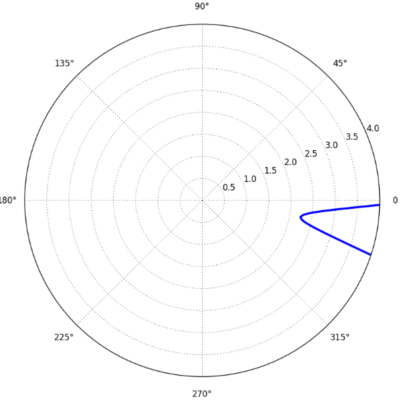
\includegraphics[width=\linewidth]{a=0dot5.png}
%  \caption{Trajectory of ray having $a = 0.5$}
%  \label{fig:result1}
% \end{figure} 
  
%\begin{figure}[h!]
%  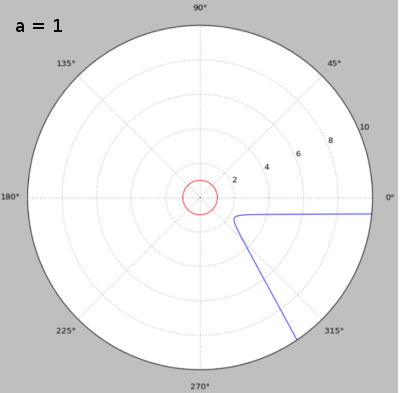
\includegraphics[width=\linewidth]{a=1.png}
% \large{ Trajectory of ray having $a = 1$}\\
%  \label{fig:result2}
%\end{figure}  
  
%\begin{figure}[h!]
%  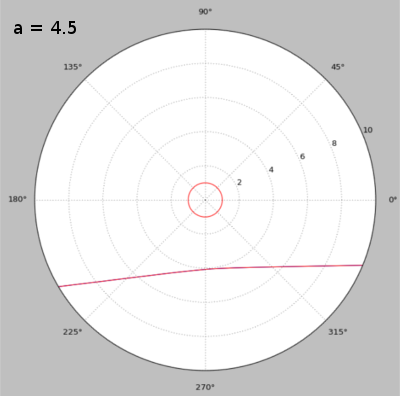
\includegraphics[width=\linewidth]{a=4dot5.png}
%  \large{ Trajectory of ray having $a=4.5$}\\  
% % \caption{Trajectory of ray having $a=4.5$}
%  \label{fig:result3}  
%\end{figure}

%\begin{figure}[h!]
%  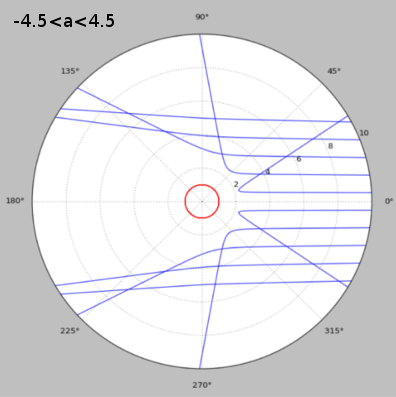
\includegraphics[width=\linewidth]{trajectory.png} 
%  \large{Trajectory of a beam which has $a$ in the range of -4.5 to +4.5}\\  
%  %\caption{Trajectory of a beam which has $a$ in the range of -4.5 to +4.5}
%  \label{fig:result4}  
%\end{figure}



\section{Calculating temperature profile of sun}
After calculating the trajectories, we will calculate the temperature(apparent brightneess temperature) of the solar corona. We will be using basic theory of radiative heat transfer. 
Consider a cool cloud as shown in Fig.4 with a hot source of radiation behind it. The radiation will enter
the cloud with intensity $I_o$, but will be absorbed on passing through the cloud.

\begin{figure}[h!]
  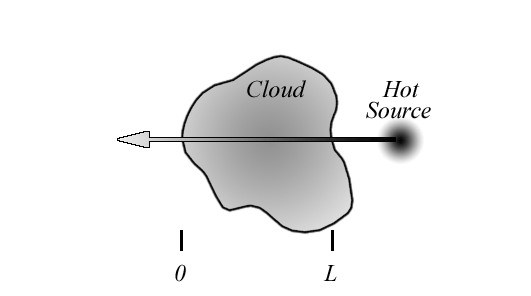
\includegraphics[width=\linewidth]{cloud.png} 
  \caption{Cloud}
  \label{fig:result4}  
\end{figure}
 

$dI = - k_nIdl$ where $I$ is the intensity entering each volume element. This is a trivial
differential equation whose solution is:
$$ I = I_0exp\Big( \int_{0}^{L}k_ndl \Big) $$ 
Note that the integration is taken along the line of sight from the observer. In the case
where the absorption is constant, of course, $k_n$ can be brought out of the integral. The
integral quantity is a dimensionless quantity called the \emph{optical depth}. The optical depth is a convenient way to refer to the "thickness" of a cloud. It measures how
many e-foldings of intensity reduction the cloud's thickness represents. \\ 

To obtain a relation between the observed temperature, source temperature and the
cloud temperature, we use the Rayleigh-Jeans approximation.

$$ T_{obs} = T_{cloud}exp(-\tau) + T_{e}(1 - exp(-\tau)) $$

\newpage


\section{Results}
The solar coronal atmosphere has been simulated using the above equations and the trajectories of the rays and the temperature profile have been plotted. All the simulations have been coded using \texttt{Python} packages like \texttt{numpy} and \texttt{scipy}.  


\vspace{2em}


We plot here the trajectories of rays with different '$a$' where $a$ denotes the distance between the ray and sun's equator at infinity. We also simulated the results when a beam of radiowave is shone on sun. We make incident a beam of rays spanning from -4.95*solar radii to  +4.95*solar radii from the sun's equator. You observe from the figure how the rays which are closer to the equator get deflected more than the rays which are far away. If we connect all the singularity points of the rays, we get the profile of sun as seen in the microwave/radiowave range i.e if we have the capability of looking at the sun in the microwave/radiowave range the sun will appear around 2.24 times than what we see now. (2.24*solar radius is the singualrity point of rays when the frequency is 10 MegaHertz).  


\begin{figure}[h!]
  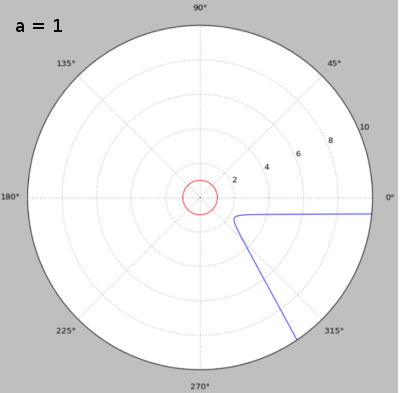
\includegraphics[width=8cm, height=8cm]{a=1.png}
 %\large{ Trajectory of ray having $a = 1$}\\
 \caption{Trajectory of ray having $a = 1$}  
  \label{fig:result2}
\end{figure}  
  
\begin{figure}[h!]
  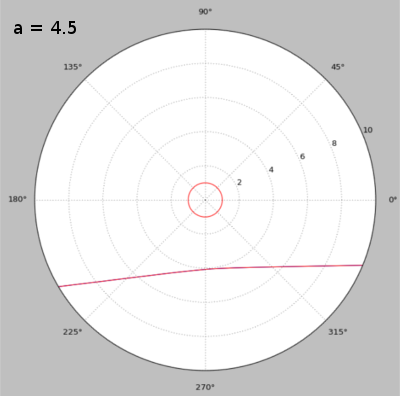
\includegraphics[width=8cm, height=8cm]{a=4dot5.png}
  %\large{ Trajectory of ray having $a=4.5$}\\  
 \caption{Trajectory of ray having $a=4.5$}
  \label{fig:result3}  
\end{figure}

\begin{figure}[h!]
  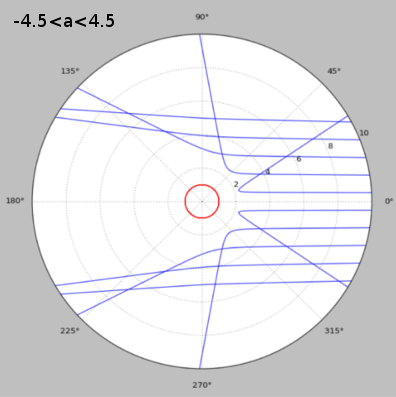
\includegraphics[width=8cm, height=8cm]{trajectory.png}  \\  
  %\large{Trajectory of a beam which has $a$ in the range of -4.5 to +4.5}\\  
  \caption{Trajectory of a beam which has $a$ in the range of -4.5 to +4.5}
  \label{fig:result4}  
\end{figure}
\vspace{10em}
\newpage


In order to calculate the temperature profile we need to calculate the optical depth as elaborated in section III. The calculation of the optical depth involves calculating the line intergral along the obtained trajectories of the individual rays. We plot the temperature profiles at different frequencies. The below displayed plots are at frequency 20 MegaHertz and 400 MegaHertz. The decreasing of the brightness temperature is due to the thinning out of electrons as the level of origin rises with decreasing frequency as observed by $[1]$

     

\begin{figure}[h!]
  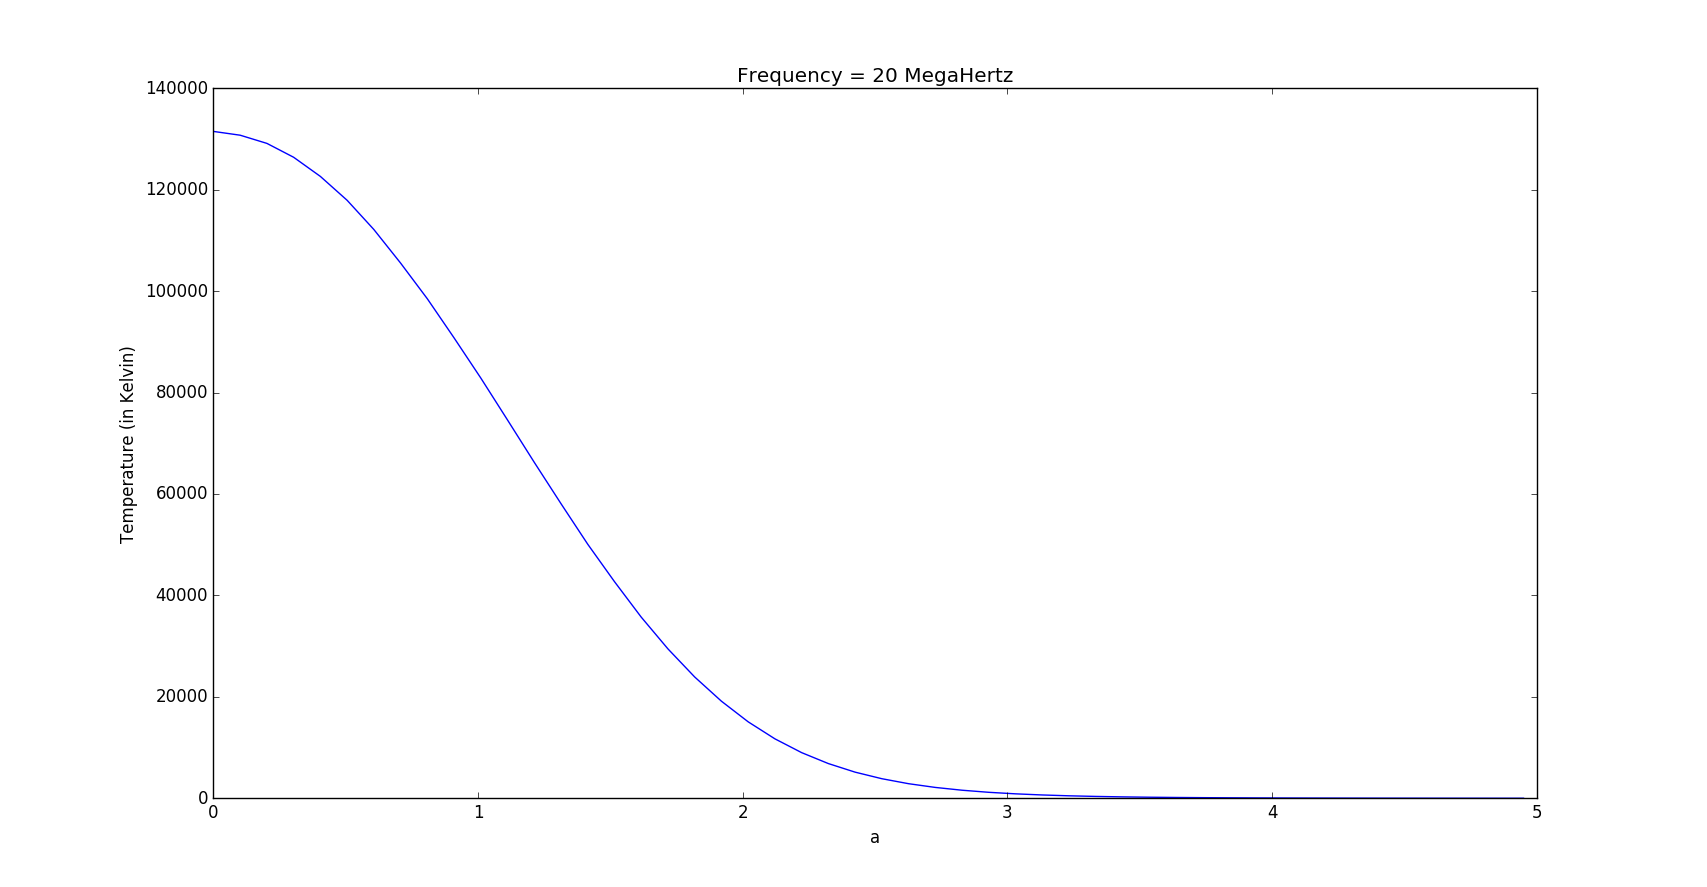
\includegraphics[width=15cm, height=10cm]{freq=20MC.png}
% \caption{Frequency = $3*10^9Hz$}\\
  \label{fig:result2}
\end{figure}  

\begin{figure}[h!]
  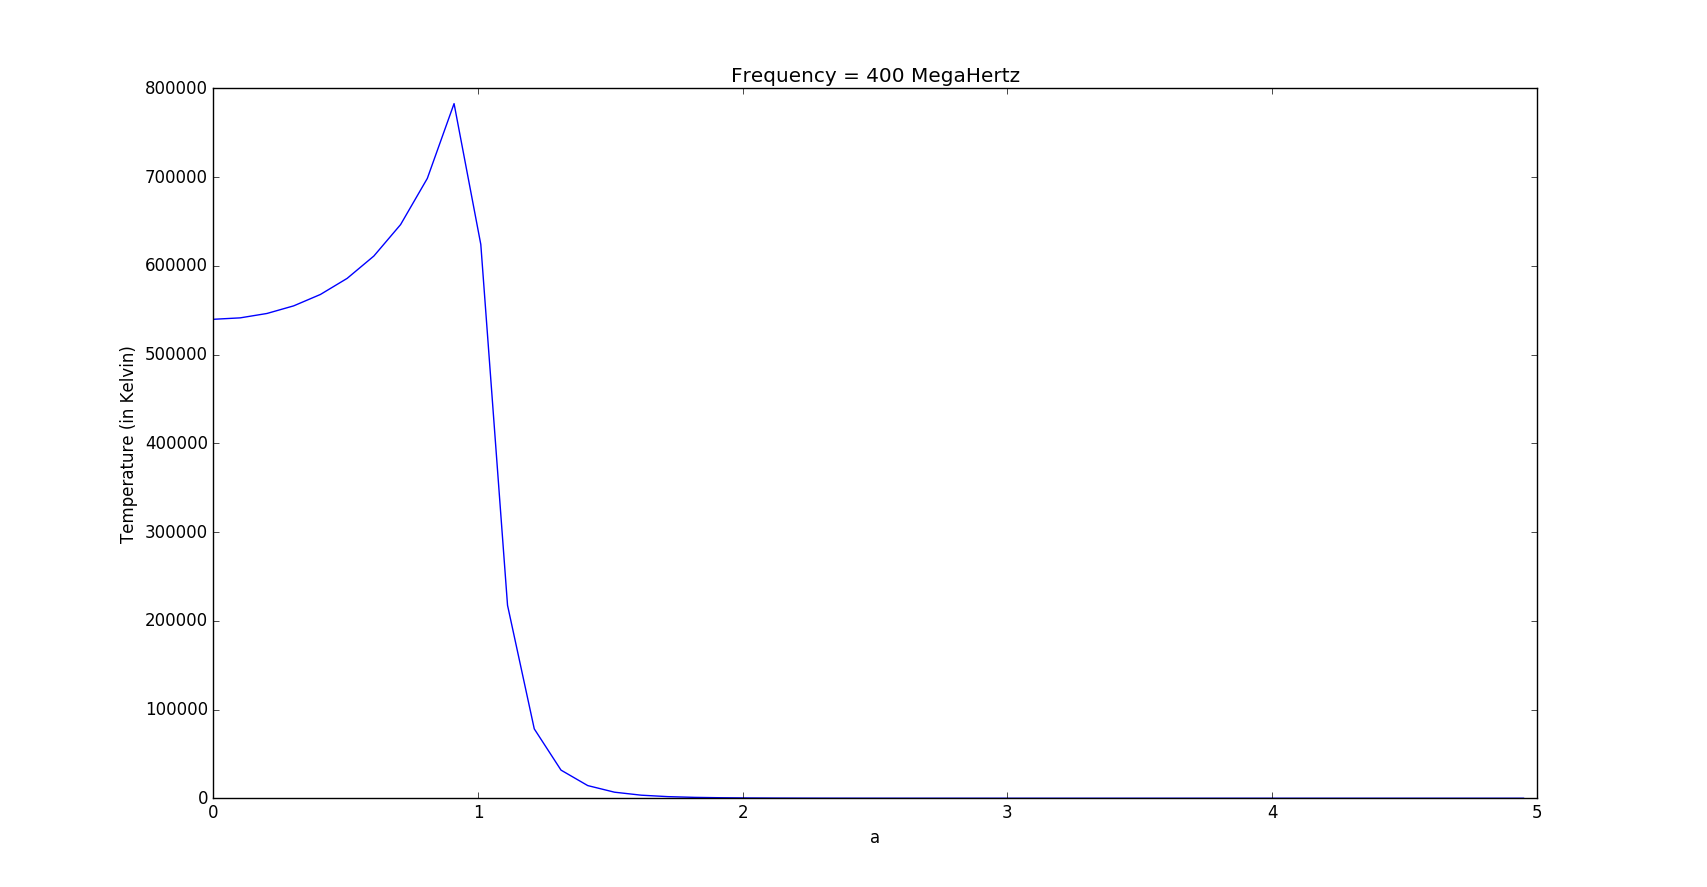
\includegraphics[width=15cm, height=10cm]{freq=400MC.png}
% \caption{Frequency = $3*10^9Hz$}\\
  \label{fig:result2}
\end{figure}  


% Can use something like this to put references on a page
% by themselves when using endfloat and the captionsoff option.
\ifCLASSOPTIONcaptionsoff
  \newpage
\fi



% trigger a \newpage just before the given reference
% number - used to balance the columns on the last page
% adjust value as needed - may need to be readjusted if
% the document is modified later
%\IEEEtriggeratref{8}
% The "triggered" command can be changed if desired:
%\IEEEtriggercmd{\enlargethispage{-5in}}

% references section

% can use a bibliography generated by BibTeX as a .bbl file
% BibTeX documentation can be easily obtained at:
% http://www.ctan.org/tex-archive/biblio/bibtex/contrib/doc/
% The IEEEtran BibTeX style support page is at:
% http://www.michaelshell.org/tex/ieeetran/bibtex/
%\bibliographystyle{IEEEtran}
% argument is your BibTeX string definitions and bibliography database(s)
%\bibliography{IEEEabrv,../bib/paper}
%
% <OR> manually copy in the resultant .bbl file
% set second argument of \begin to the number of references
% (used to reserve space for the reference number labels box)

% biography section
% 
% If you have an EPS/PDF photo (graphicx package needed) extra braces are
% needed around the contents of the optional argument to biography to prevent
% the LaTeX parser from getting confused when it sees the complicated
% \includegraphics command within an optional argument. (You could create
% your own custom macro containing the \includegraphics command to make things
% simpler here.)
%\begin{biography}[{\includegraphics[width=1in,height=1.25in,clip,keepaspectratio]{mshell}}]{Michael Shell}
% or if you just want to reserve a space for a photo:

%\begin{IEEEbiography}[{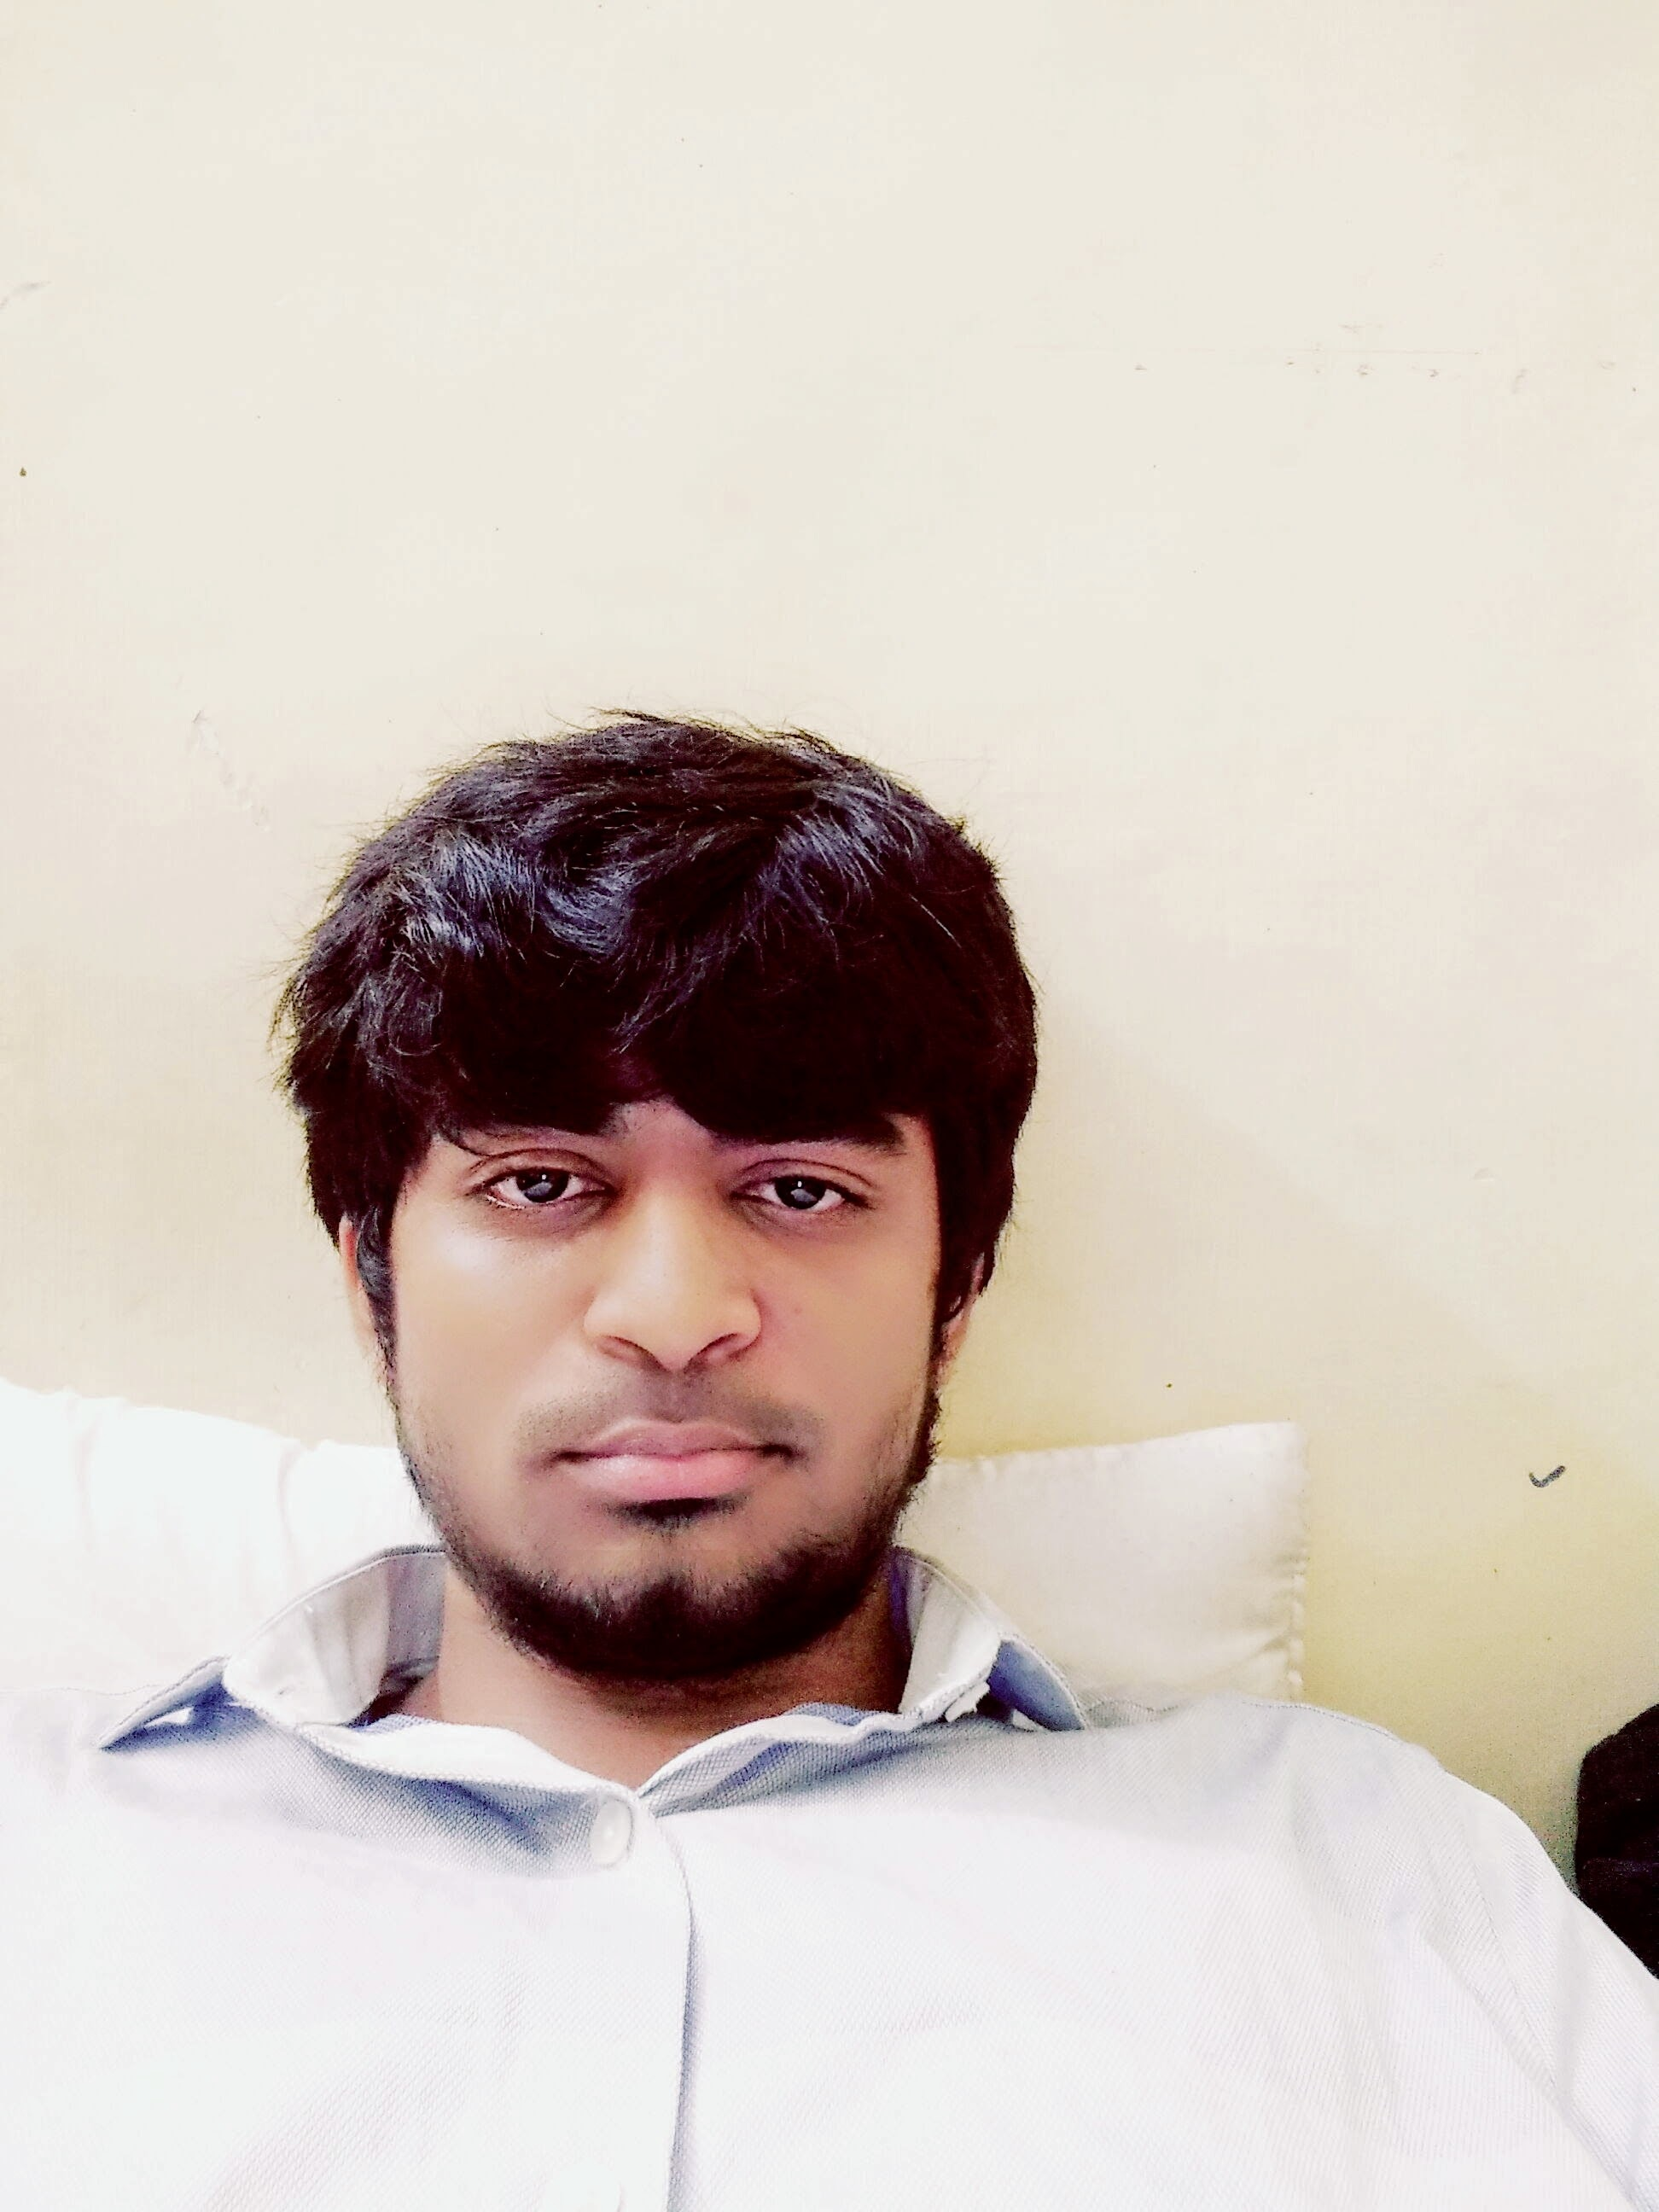
\includegraphics[width=1in,height=1.25in,clip,keepaspectratio]{picture}}]{Pranav Sankhe}
%I am a 3rd-year undergraduate student at the Electrical Engineering Department of Indian Institute of Technology, Bombay. I am passionate about Deep Learning, Computer Vision, Optimization, Computational Neuroscience, Neuromorphic Modeling and Distributed Wireless Networks. 
%\end{IEEEbiography}

% You can push biographies down or up by placing
% a \vfill before or after them. The appropriate
% use of \vfill depends on what kind of text is
% on the last page and whether or not the columns
% are being equalized.

%\vfill

% Can be used to pull up biographies so that the bottom of the last one
% is flush with the other column.
%\enlargethispage{-5in}



% that's all folks
\end{document}


